Recently, many researchers have become more interested in applying deep learning techniques to communications systems.  
We refer the reader to \cite{botoca}\cite{diamandis}\cite{wang}\cite{hemodel}\cite{osheaphys} for surveys and motivations of these kind of works.  
Most of the works that we have found typically only deal with additive white gaussian noise (AWGN) channels or Rayleigh fading channels.

In \cite{dorner2017}, D\"{o}rner et. al. implemented an end to end transmitter and reciever with neural networks that allowed gradients to flow all the way back from the receiver during training.  
However, they restricted themselves to only sending a certain set of messages, only seeing AWGN channels, and they did not address CFO. 

Other groups have been focusing on decoding with recurrent neural networks (RNNs) but also only deal with AWGN channels \cite{kim2018}\cite{kimnips}.  
Others have been working with generative adversarial networks (GANs) to train an end-to-end communication system \cite{yegans}.  However, they also only consider AWGN channels or Rayleigh fading channels.

For those that do consider more complex channels, most re-train their models for each new channel seen.  Ye et. al. consider OFDM systems where their feedforward neural networks estimate the channel state information and then train offline for that specific channel \cite{ye2018}.  
\cite{raghavendra} considers nonlinear channels but re-trains the network for each new channel.  Note, this work does not go into detail about the architecture used or how the networks are trained. 

Goldsmith and Farsad train a detector for optical and moleculular channels \cite{farsad2018}.  They assume a Poisson model for the channel and attempt to predict the probability mass function.  However, they assume that they retrain for each Poisson parameter and they do not address CFO.

Timothy O'Shea's group has been doing some excellent work in this area. 
O'Shea's first work in this area jointly optimized a transmitter and receiver for a given channel model (AWGN and Rayleigh fading) but the work does not go into detail about the performance for various channels \cite{osheaphys}.

In a subsequent paper, O'Shea et. al. explored how multipath channels and random initial phase affects the system performance \cite{osheaatt}.  
This is the only work that we know of that does not re-train for each new multipath channel or carrier frequency offset. 
Figure~\ref{fig:oshea} shows how the convolutional neural network performance drastically decreased with multipath channels and for non-zero phase offset.
This particularly motivates our work as we hope to increase performance on learning to learn equalization and CFO.

\begin{figure}
\begin{center}
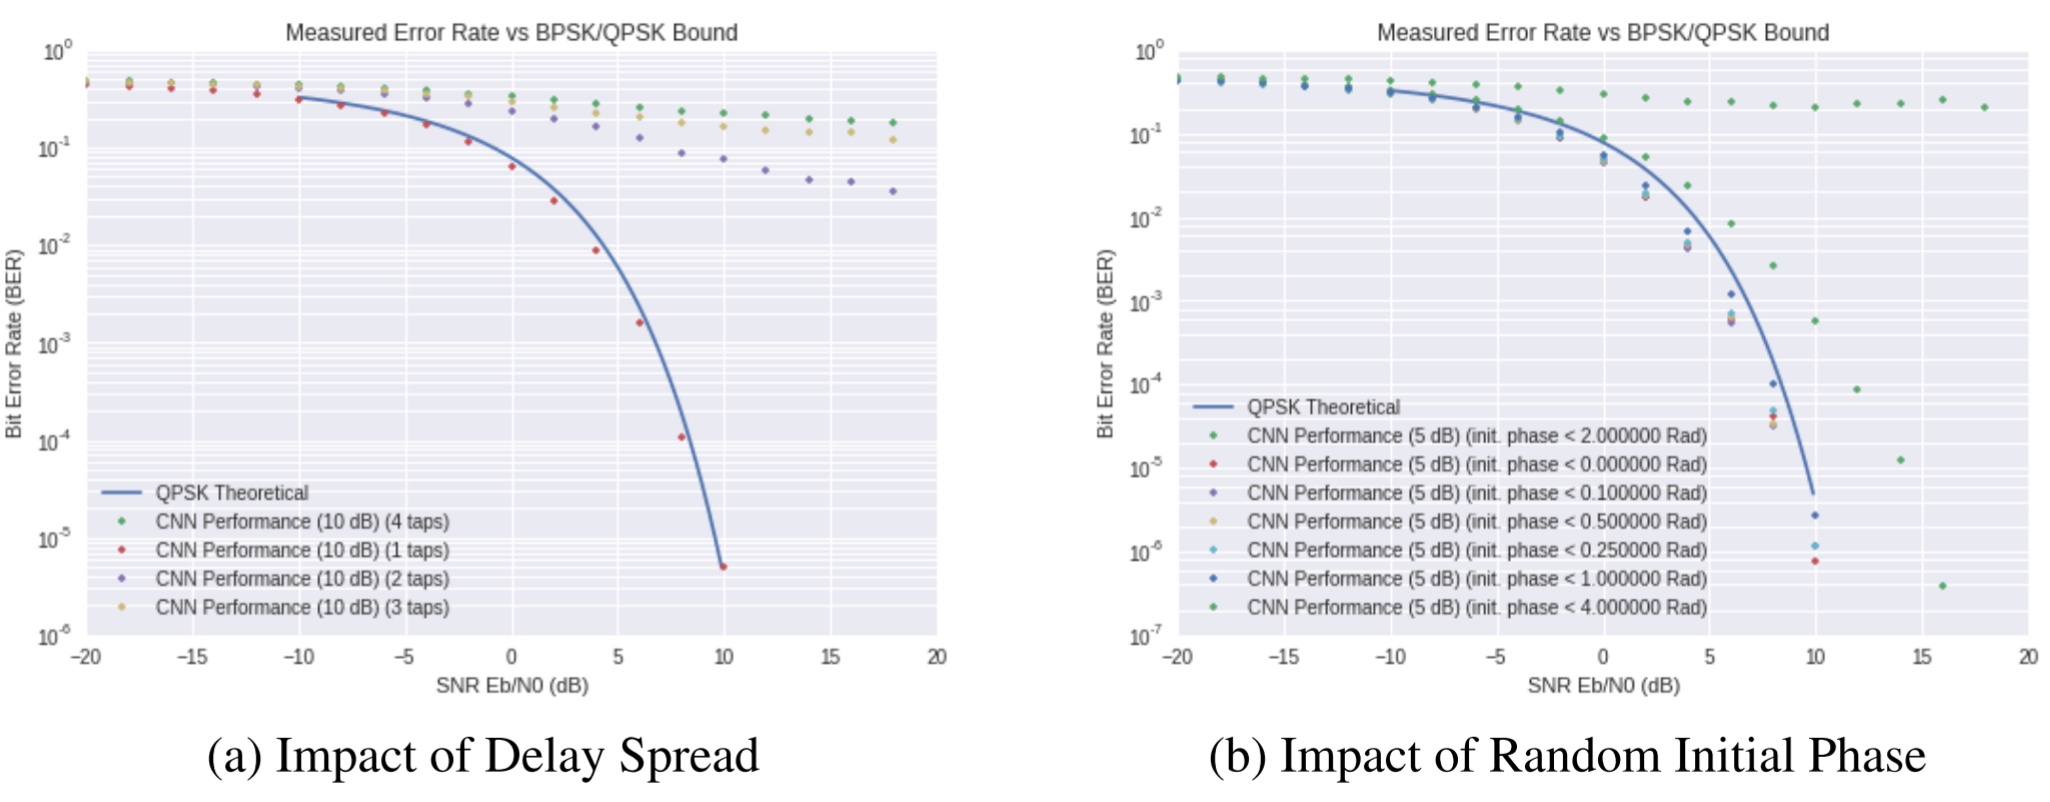
\includegraphics[width=16cm]{figures/osheaatt2.png}
\caption{The impacts of multipath channels and initial phase offsets on bit error performance \cite{osheaatt}.  Note, the network is not re-trained for each new environment.  As the number of paths and carrier frequency offset increase, the performance of the CNN decreases.}
\label{fig:oshea}
\end{center}
\end{figure}

In \cite{osheasynch}, they added an attention model to perform synchronization for time, frequency, phase, and sample timing offset.  However, their work showed that the synchronization was still quite noisy and did not perform much better than without the attention model \cite{osheaatt}.  Additionally, this work did not consider multipath channels. 

O'Shea et. al. have also attempted to use GANs to approxiate the channel response model for AWGN channels with and without phase noise \cite{osheavoid}.  The GANs were unable to find accurate probability density functions to represent the channel response.  

In \cite{osheacsi}, they use convolutional neural networks (CNNs) to estimate, but not correct, carrier frequency offset and timing offset.  However, they only consider AWGN channels and Rayleigh fading channels.  
In \cite{osheamimo}, they explore how unsupervised learning can train autoencoders for multiple antenna communications.  They do re-train for each new channel and use a Rayleigh fading channel model.
